\chapter{Phân loại FashionMNIST bằng ANN}

\section{Tổng quan}

Sau khi hoàn tất chuỗi thí nghiệm trên MNIST Handwritten, các mô hình ANN được chuyển sang FashionMNIST để kiểm tra khả năng tổng quát hóa trên một bộ dữ liệu khó hơn~\cite{xiao2017fashion,fashionmnist_repo}. Nếu MNIST chủ yếu khác nhau ở hướng nét và bố cục stroke, thì FashionMNIST khó hơn ở chỗ nhiều lớp có silhouette gần nhau, đặc biệt giữa \textit{T-shirt/top}, \textit{Shirt}, \textit{Pullover} và \textit{Coat}. Vì vậy, chương này cũng giữ đúng tinh thần của Chương 1: bắt đầu từ baseline naive chỉ dùng raw pixel, sau đó tăng dần mức độ đặc trưng hóa và độ ổn định dự đoán để xem yếu tố nào thực sự có ích trên dữ liệu thời trang.

\section{Phát biểu bài toán}

Bài toán cần giải quyết là phân lớp ảnh thời trang thành $10$ lớp như \textit{T-shirt/top}, \textit{Trouser}, \textit{Pullover}, \textit{Dress}, \textit{Coat}, \textit{Sandal}, \textit{Shirt}, \textit{Sneaker}, \textit{Bag} và \textit{Ankle boot}. Đầu vào của mô hình là ảnh xám kích thước $28 \times 28$, nên mỗi mẫu gốc có $784$ pixel. Đầu ra vẫn là vector logits $10$ chiều; lớp có logit lớn nhất được chọn làm nhãn dự đoán cuối cùng.

Về mặt dữ liệu, FashionMNIST cũng là bài toán \textit{single-label classification}. Trong Lab 03, dữ liệu được dùng theo đúng hai split chính thức của bộ dữ liệu: $60{,}000$ mẫu train để huấn luyện và $10{,}000$ mẫu test để đánh giá cuối~\cite{xiao2017fashion}. Không có validation riêng được tách ra, nên toàn bộ so sánh giữa các mô hình trong chương này đều bám trên cùng một protocol train/test.

\begin{table}[H]
\centering
\caption{Phát biểu bài toán và thiết lập dữ liệu của FashionMNIST}
\label{tab:fashion-mnist-problem-setup}
\begin{tabular}{l c}
\toprule
Thành phần & Giá trị \\
\midrule
Kiểu bài toán & Single-label classification \\
Đầu vào & Ảnh xám $28 \times 28$ \\
Đầu ra & Vector logits $10$ chiều \\
Số lớp & $10$ lớp thời trang \\
Train chính thức & $60{,}000$ mẫu \\
Test chính thức & $10{,}000$ mẫu \\
Thiết lập Lab 03 & Dùng toàn bộ train để huấn luyện, test ở cuối \\
\bottomrule
\end{tabular}
\end{table}


\section{Mô hình và tham số}
\subsection{Naive ANN}

Naive ANN là baseline tối giản nhất của chương này và cũng là điểm xuất phát cần thiết để kiểm tra xem ANN thuần có thể đi được đến đâu nếu chỉ nhìn ảnh thời trang ở mức pixel thô. Đầu vào của mô hình chỉ gồm raw pixel được trải phẳng thành vector $784$ chiều, hoàn toàn không có \textit{deslant}, \textit{recenter}, HOG hay bất kỳ augmentation nào. Lớp vào vì thế có đúng $784$ neuron, tương ứng trực tiếp với $784$ pixel của ảnh xám $28 \times 28$. Đầu ra là vector logits $10$ chiều để biểu diễn mười lớp trang phục; lớp có logit lớn nhất được chọn làm dự đoán cuối cùng.

Kiến trúc MLP được giữ cùng khuôn với baseline ở Chương 1:
\[
784 \rightarrow 1024 \rightarrow 512 \rightarrow 256 \rightarrow 10.
\]
Ba tầng ẩn dùng ReLU, còn hàm mất mát là \textit{cross-entropy} tiêu chuẩn. Cách chọn số chiều ẩn cũng mang cùng triết lý như ở MNIST: tầng đầu mở rộng lên $1024$ để mô hình có đủ không gian kết hợp các pixel thô thành những biểu diễn giàu hơn; hai tầng sau giảm dần về $512$ rồi $256$ để nén dần biểu diễn trước khi đi tới lớp phân loại. Việc không tiếp tục làm các tầng sau ngày càng rộng hơn giúp baseline tránh tăng quá mạnh số tham số trong khi đầu vào vẫn còn rất thô và thiếu cấu trúc. Optimizer được chọn là Adam để baseline hội tụ ổn định mà không thêm các kỹ thuật regularization phụ. Mục tiêu của biến thể này là trả lời trực tiếp câu hỏi: nếu chỉ dùng pixel thô, ANN có thể đi được tới đâu trên FashionMNIST.

\begin{table}[H]
\centering
\caption{Kết quả của naive ANN trên FashionMNIST}
\label{tab:fashion-mnist-naive-results}
\begin{tabular}{l c}
\toprule
Chỉ số & Giá trị \\
\midrule
Final train accuracy & 0.9796 \\
Test accuracy & 0.8959 \\
Generalization gap & 0.0837 \\
\bottomrule
\end{tabular}
\end{table}


\begin{figure}[H]
  \centering
  
\includegraphics[width=0.95\textwidth]{figures/fashion-mnist-naive/training_curves.png}
  \caption{Diễn biến train accuracy và train loss của naive ANN trên FashionMNIST trong 50 epoch.}
  \label{fig:fashion-mnist-naive-training-curves}
\end{figure}

\begin{figure}[H]
  \centering
  
\includegraphics[width=0.82\textwidth]{figures/fashion-mnist-naive/confusion_matrix.png}
  \caption{Confusion matrix của naive ANN trên FashionMNIST.}
  \label{fig:fashion-mnist-naive-confusion}
\end{figure}

\begin{figure}[H]
  \centering
  
\includegraphics[width=0.95\textwidth]{figures/fashion-mnist-naive/class_accuracy_bar.png}
  \caption{Accuracy theo từng lớp của naive ANN trên FashionMNIST.}
  \label{fig:fashion-mnist-naive-class-accuracy}
\end{figure}

\begin{table}[H]
\centering
\caption{Các cặp nhầm lẫn lớn nhất của naive ANN trên FashionMNIST}
\label{tab:fashion-mnist-naive-top-errors}
\begin{tabular}{l c}
\toprule
Cặp nhầm lẫn & Số mẫu \\
\midrule
T-shirt/top $\rightarrow$ Shirt & 125 \\
Shirt $\rightarrow$ T-shirt/top & 103 \\
Coat $\rightarrow$ Pullover & 101 \\
Pullover $\rightarrow$ Shirt & 79 \\
Coat $\rightarrow$ Shirt & 79 \\
Shirt $\rightarrow$ Pullover & 72 \\
Pullover $\rightarrow$ Coat & 56 \\
Ankle boot $\rightarrow$ Sneaker & 46 \\
\bottomrule
\end{tabular}
\end{table}


Naive ANN đạt $89.59\%$ test accuracy. Các cặp nhầm lẫn lớn nhất đã lộ ra rất rõ ngay từ baseline: \textit{T-shirt/top} $\rightarrow$ \textit{Shirt}, \textit{Shirt} $\rightarrow$ \textit{T-shirt/top}, \textit{Coat} $\rightarrow$ \textit{Pullover}, \textit{Pullover} $\rightarrow$ \textit{Shirt}. Điều này cho thấy với FashionMNIST, raw pixel đơn thuần chưa đủ để tách các lớp có hình dáng gần nhau, nhất là khi khác biệt nằm ở hướng biên, nếp áo và phân bố hình học tổng thể.

Từ kết quả này, bước tiếp theo hợp lý là thêm chuẩn hóa hình học và đặc trưng gradient để mô hình không chỉ nhìn cường độ pixel thô, mà còn nắm rõ hướng nét và cấu trúc biên của từng loại trang phục.

\subsection{Single-branch ANN}

Single-branch ANN là biến thể cải tiến trực tiếp từ baseline naive. Điểm xuất phát của biến thể này là insight vừa rút ra: raw pixel thuần chưa đủ để tách các lớp quần áo có silhouette gần nhau, nên mô hình cần được bổ sung thông tin hình học và hướng biên ngay từ đầu. Vì vậy, ảnh trước hết được chuẩn hóa bằng \textit{deslant + recenter} để làm ổn định bố cục tổng thể, sau đó biểu diễn đầu vào được mở rộng thành vector $2080 = 784 + 1296$ chiều, trong đó $784$ chiều đến từ raw pixel sau tiền xử lý và $1296$ chiều đến từ HOG. MLP phía sau có dạng:
\[
2080 \rightarrow 1024 \rightarrow 512 \rightarrow 256 \rightarrow 10.
\]
Ba tầng ẩn dùng BatchNorm, GELU và Dropout$(0.25)$. Kích thước $1024 \rightarrow 512 \rightarrow 256$ được giữ nguyên từ Chương 1 vì mục tiêu ở đây là kiểm tra khả năng chuyển giao của cấu hình mạnh nhất trên MNIST sang dữ liệu thời trang, thay vì thay đổi quá nhiều thành phần cùng lúc. Tầng đầu giữ ở mức $1024$ để hấp thụ đầu vào $2080$ chiều sau khi ghép raw pixel và HOG; các tầng sau tiếp tục giảm dần để nén biểu diễn và giữ cho phần phân loại cuối đủ gọn. BatchNorm được dùng để ổn định kích hoạt khi đầu vào đã là sự kết hợp của hai nguồn đặc trưng khác bản chất, còn Dropout được thêm để giảm độ nhạy của các lớp fully-connected tương đối rộng. Loss tiếp tục là \textit{cross-entropy} có \textit{label smoothing} $0.05$, còn optimizer là AdamW với cosine scheduler nhằm giữ quá trình tối ưu ổn định hơn so với baseline.

\begin{table}[H]
\centering
\caption{Kết quả single-branch ANN trên FashionMNIST}
\label{tab:fashion-mnist-single-branch-results}
\begin{tabular}{l c}
\toprule
Chỉ số & Giá trị \\
\midrule
Final train accuracy & 0.99997 \\
Final train loss & 0.2906 \\
Test accuracy & 0.9060 \\
Generalization gap & 0.0940 \\
Epochs & 50 \\
\bottomrule
\end{tabular}
\end{table}


\begin{figure}[H]
  \centering
  
\includegraphics[width=0.95\textwidth]{figures/fashion-mnist-ann/training_curves.png}
  \caption{Diễn biến train accuracy và train loss của single-branch ANN trên FashionMNIST trong 50 epoch.}
  \label{fig:fashion-mnist-training-curves}
\end{figure}

\begin{figure}[H]
  \centering
  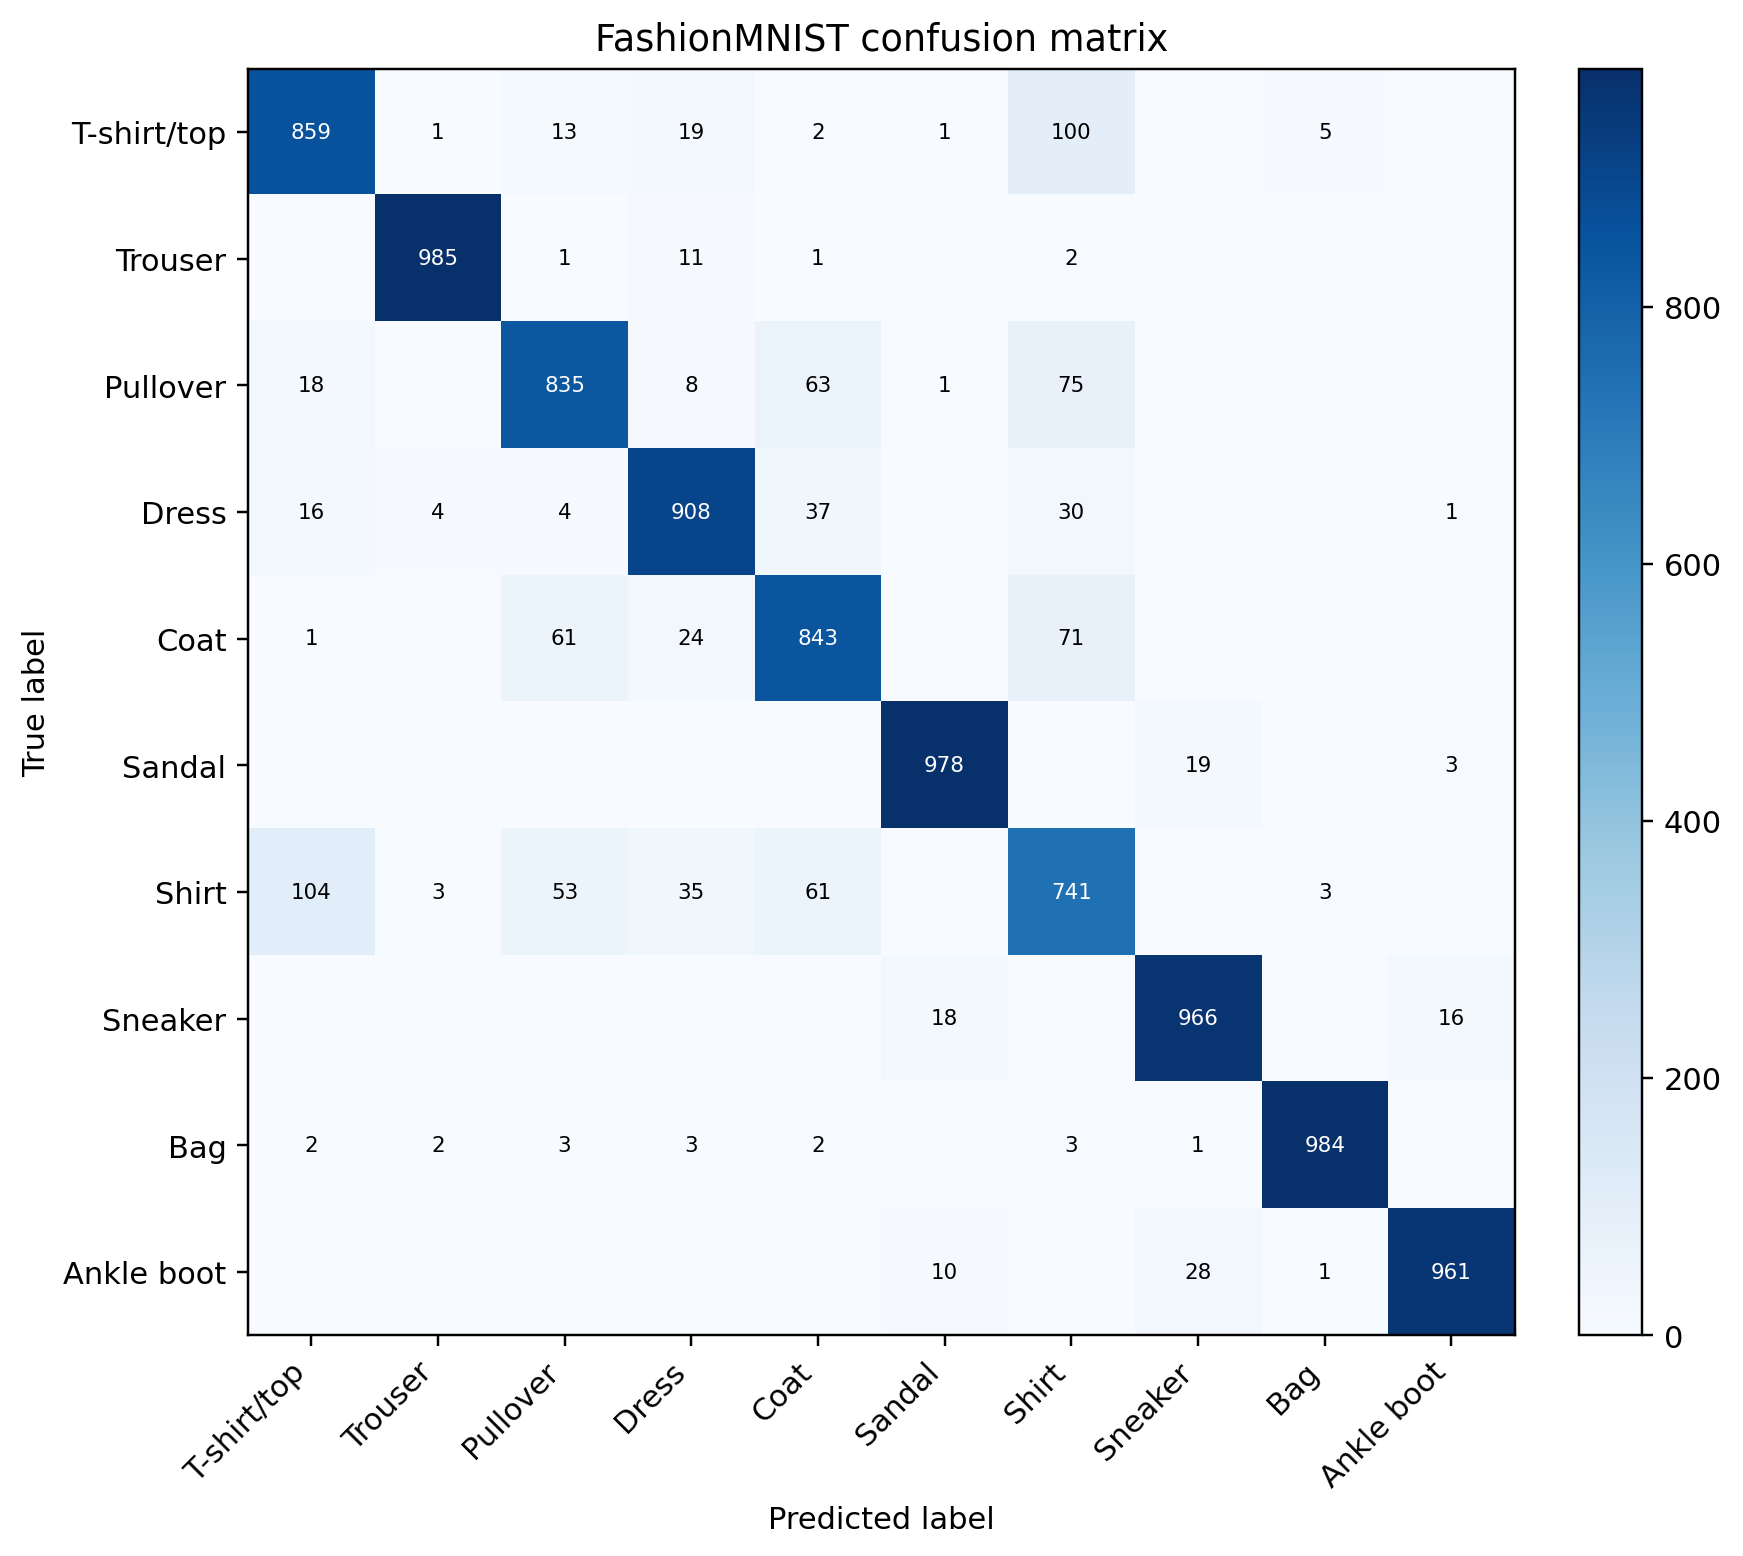
\includegraphics[width=0.82\textwidth]{figures/fashion-mnist-ann/confusion_matrix.png}
  \caption{Confusion matrix của single-branch ANN trên FashionMNIST.}
  \label{fig:fashion-mnist-confusion}
\end{figure}

\begin{figure}[H]
  \centering
  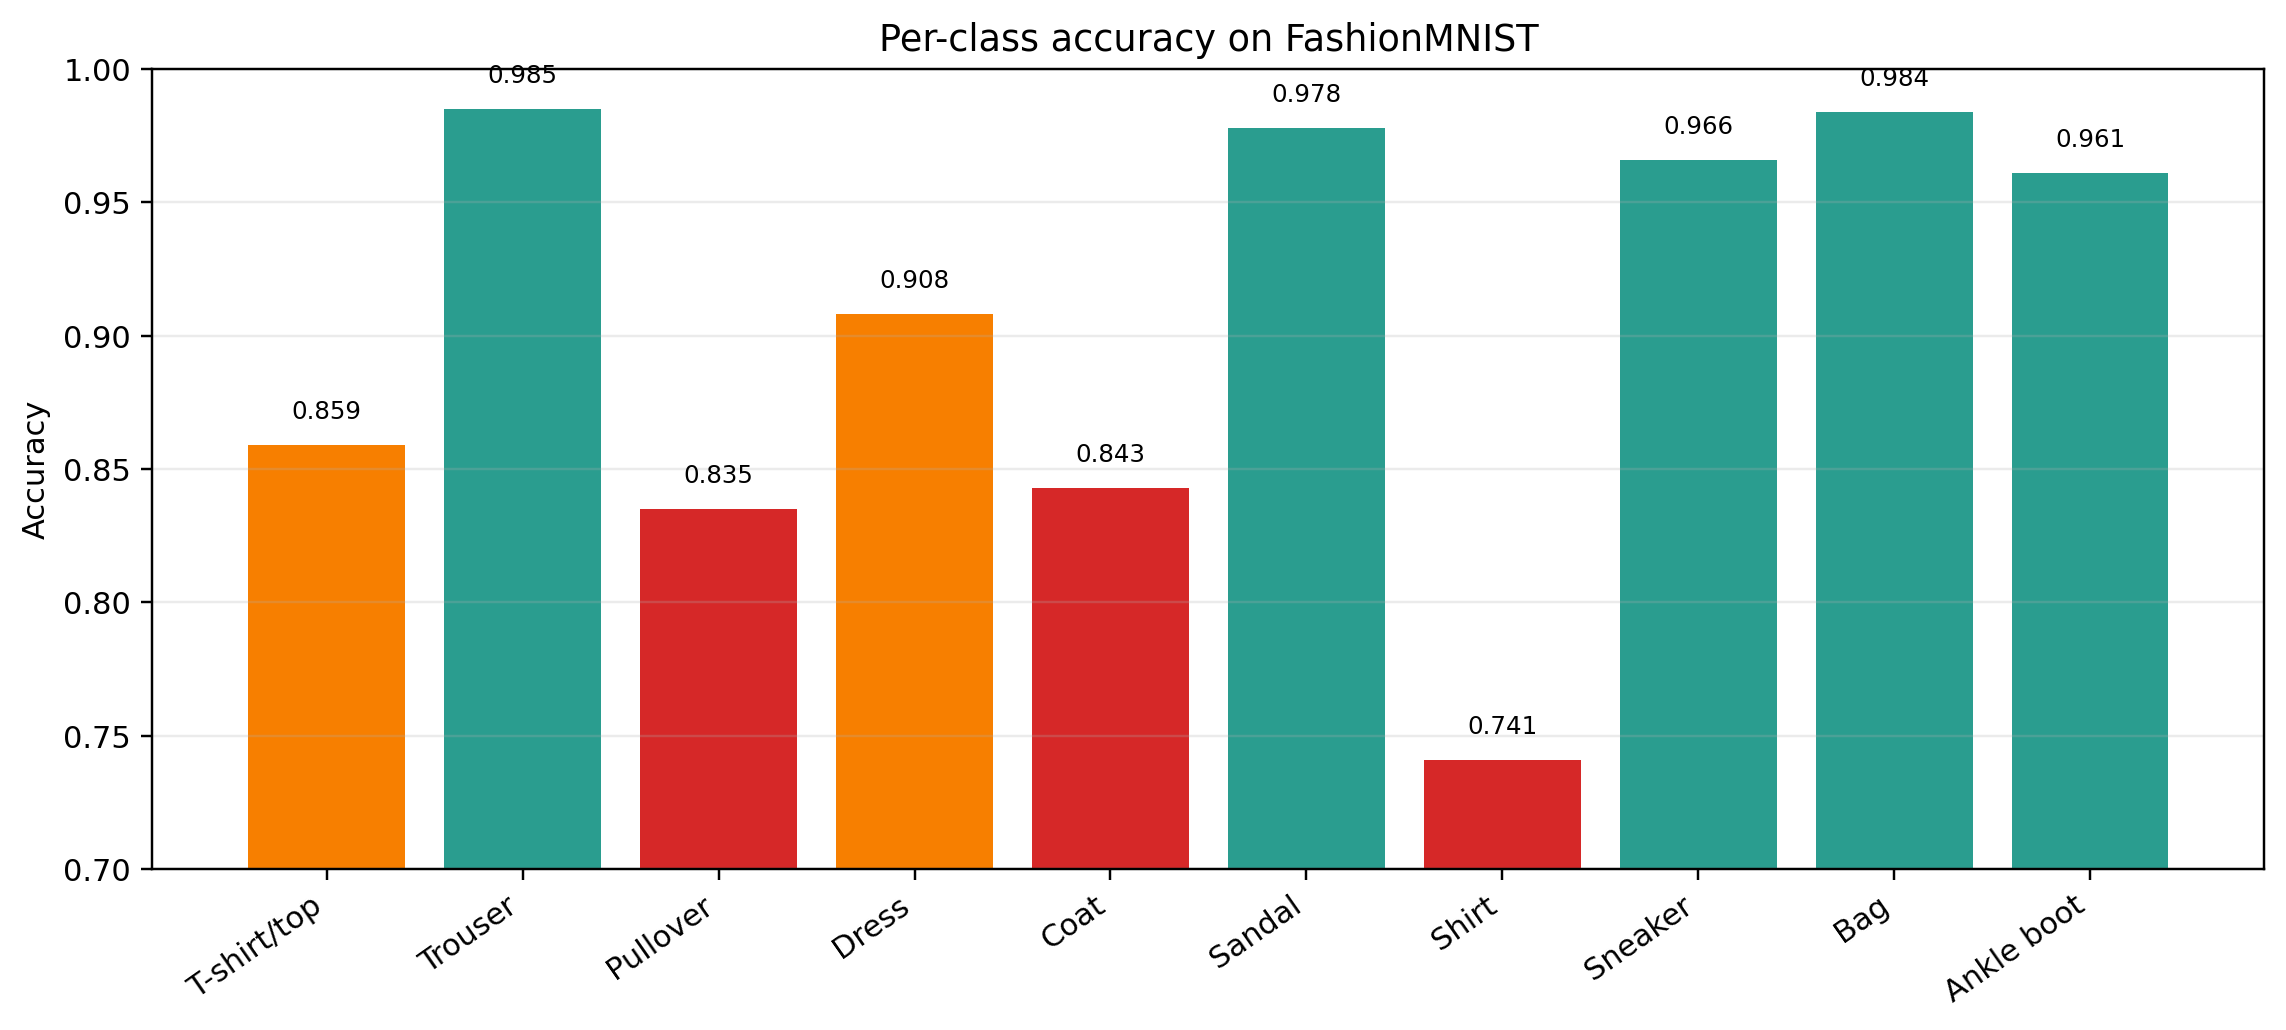
\includegraphics[width=0.95\textwidth]{figures/fashion-mnist-ann/class_accuracy_bar.png}
  \caption{Accuracy theo từng lớp của single-branch ANN trên FashionMNIST.}
  \label{fig:fashion-mnist-class-accuracy}
\end{figure}

\begin{table}[H]
\centering
\caption{Các cặp nhầm lẫn lớn nhất của single-branch ANN trên FashionMNIST}
\label{tab:fashion-mnist-top-errors}
\begin{tabular}{l c}
\toprule
Cặp nhầm lẫn & Số mẫu \\
\midrule
Shirt $\rightarrow$ T-shirt/top & 104 \\
T-shirt/top $\rightarrow$ Shirt & 100 \\
Pullover $\rightarrow$ Shirt & 75 \\
Coat $\rightarrow$ Shirt & 71 \\
Pullover $\rightarrow$ Coat & 63 \\
Shirt $\rightarrow$ Coat & 61 \\
Coat $\rightarrow$ Pullover & 61 \\
Shirt $\rightarrow$ Pullover & 53 \\
\bottomrule
\end{tabular}
\end{table}


Single-branch ANN đạt \textit{test accuracy} $90.60\%$ với \textit{generalization gap} khoảng $9.4\%$, thấp hơn đáng kể so với mức hơn $99\%$ trên MNIST. Confusion matrix và bảng top lỗi cho thấy khó khăn tập trung mạnh vào các lớp áo có hình dáng gần nhau, nổi bật nhất là \textit{Shirt} $\rightarrow$ \textit{T-shirt/top}, \textit{T-shirt/top} $\rightarrow$ \textit{Shirt}, \textit{Pullover} $\rightarrow$ \textit{Shirt} và \textit{Coat} $\rightarrow$ \textit{Shirt}. Điều này cho thấy với FashionMNIST, đặc trưng hình học cơ bản đã giúp nhiều nhưng vẫn chưa đủ để tách các lớp chồng lấn mạnh về silhouette.

Từ kết quả này, giả thuyết kế tiếp là: nếu raw pixel và HOG đang bị hòa trộn quá sớm ở đầu vào chung, có thể việc tách chúng thành hai nhánh riêng sẽ giúp mỗi nguồn đặc trưng học vai trò chuyên biệt hơn trước khi hợp nhất.

\subsection{Two-branch ANN}

Two-branch ANN dùng cùng đầu vào và cùng pipeline \textit{deslant + recenter + HOG} như single-branch, nhưng thay vì ghép raw pixel và HOG ngay từ đầu, mô hình tách chúng thành hai nhánh riêng. Insight dẫn tới biến thể này là: nếu raw pixel và HOG có vai trò khác nhau, việc ép chúng đi qua cùng một tầng đầu có thể làm thông tin bị hòa trộn quá sớm. Vì vậy, nhánh raw có dạng $784 \rightarrow 512 \rightarrow 256$, nhánh HOG có dạng $1296 \rightarrow 768 \rightarrow 256$, sau đó hai vector $256$ chiều được ghép lại thành $512$ chiều và đi qua head cuối:
\[
512 \rightarrow 256 \rightarrow 10.
\]
Ý tưởng của biến thể này hoàn toàn giống Chương 1: raw pixel và HOG có bản chất khác nhau, nên có thể có lợi nếu cho chúng học biểu diễn riêng trước khi hợp nhất. Nhánh HOG được cấp tầng đầu rộng hơn vì đầu vào của nó nhiều chiều hơn và mang sẵn thông tin cấu trúc mạnh hơn raw pixel; cả hai nhánh đều được nén về $256$ chiều để quá trình hợp nhất ở phần head không bị lệch hẳn về một bên.

\begin{table}[H]
\centering
\caption{Kết quả two-branch ANN trên FashionMNIST}
\label{tab:fashion-mnist-two-branch-results}
\begin{tabular}{l c}
\toprule
Chỉ số & Giá trị \\
\midrule
Final train accuracy & 0.99987 \\
Final train loss & 0.2918 \\
Test accuracy & 0.8969 \\
Generalization gap & 0.1030 \\
Epochs & 50 \\
\bottomrule
\end{tabular}
\end{table}


\begin{figure}[H]
  \centering
  
\includegraphics[width=0.95\textwidth]{figures/fashion-mnist-two-branch/training_curves.png}
  \caption{Diễn biến train accuracy và train loss của two-branch ANN trên FashionMNIST trong 50 epoch.}
  \label{fig:fashion-mnist-two-branch-training-curves}
\end{figure}

\begin{figure}[H]
  \centering
  
\includegraphics[width=0.82\textwidth]{figures/fashion-mnist-two-branch/confusion_matrix.png}
  \caption{Confusion matrix của two-branch ANN trên FashionMNIST.}
  \label{fig:fashion-mnist-two-branch-confusion}
\end{figure}

\begin{figure}[H]
  \centering
  
\includegraphics[width=0.95\textwidth]{figures/fashion-mnist-two-branch/class_accuracy_bar.png}
  \caption{Accuracy theo từng lớp của two-branch ANN trên FashionMNIST.}
  \label{fig:fashion-mnist-two-branch-class-accuracy}
\end{figure}

\begin{table}[H]
\centering
\caption{Các cặp nhầm lẫn lớn nhất của two-branch ANN trên FashionMNIST}
\label{tab:fashion-mnist-two-branch-top-errors}
\begin{tabular}{l c}
\toprule
Cặp nhầm lẫn & Số mẫu \\
\midrule
T-shirt/top $\rightarrow$ Shirt & 120 \\
Shirt $\rightarrow$ T-shirt/top & 102 \\
Pullover $\rightarrow$ Shirt & 87 \\
Coat $\rightarrow$ Shirt & 80 \\
Coat $\rightarrow$ Pullover & 70 \\
Shirt $\rightarrow$ Coat & 62 \\
Shirt $\rightarrow$ Pullover & 57 \\
Pullover $\rightarrow$ Coat & 49 \\
\bottomrule
\end{tabular}
\end{table}


Two-branch ANN chỉ đạt $89.69\%$ test accuracy và có \textit{generalization gap} khoảng $10.3\%$, tức còn thấp hơn single-branch. Mẫu lỗi vẫn gần như giữ nguyên: \textit{T-shirt/top} $\leftrightarrow$ \textit{Shirt}, \textit{Pullover} $\rightarrow$ \textit{Shirt}, \textit{Coat} $\rightarrow$ \textit{Shirt}. Điều này cho thấy trên FashionMNIST, bottleneck không còn nằm ở chỗ raw pixel và HOG có bị ghép quá sớm hay không; khó khăn chính là ranh giới lớp chồng lấn mạnh, và việc tăng độ phức tạp của kiến trúc chưa đủ để giải quyết.

Từ đây, hướng đi hợp lý hơn là không cố làm kiến trúc phức tạp hơn nữa, mà giữ biến thể đơn tốt nhất rồi giảm phương sai dự đoán bằng ensemble nhiều seed.

\subsection{Ensemble các mô hình single-branch}

Sau khi two-branch không cải thiện, bước tiếp theo không còn là làm kiến trúc phức tạp hơn, mà là kiểm tra xem single-branch có đang bị giới hạn bởi phương sai do khởi tạo và thứ tự mini-batch hay không. Vì vậy, biến thể này giữ nguyên toàn bộ cấu hình single-branch tốt nhất của chương: cùng đầu vào $2080 = 784 + 1296$, cùng kiến trúc
\[
2080 \rightarrow 1024 \rightarrow 512 \rightarrow 256 \rightarrow 10,
\]
cùng BatchNorm, GELU, Dropout$(0.25)$, AdamW, cross-entropy với label smoothing và cosine scheduler. Mô hình được huấn luyện độc lập ba lần với seed $42$, $52$ và $62$.

Động lực học của lựa chọn này khá trực tiếp: nếu mỗi mô hình đơn đã học được đặc trưng tương đối tốt nhưng nghiệm tối ưu cuối cùng còn nhạy với seed, thì việc lấy trung bình xác suất softmax ở bước test sẽ giúp làm phẳng dao động giữa các nghiệm đó. Nói cách khác, ensemble ở đây không nhằm thay đổi biểu diễn đầu vào, mà nhằm giảm phương sai dự đoán trong khi vẫn giữ nguyên biến thể đơn tốt nhất để so sánh công bằng.

\begin{table}[H]
\centering
\caption{Ba mô hình thành phần trong ensemble single-branch ANN trên FashionMNIST}
\label{tab:fashion-mnist-ensemble-member-details}
\small
\begin{tabularx}{\textwidth}{>{\raggedright\arraybackslash}p{2.2cm} >{\raggedright\arraybackslash}p{1.4cm} >{\raggedright\arraybackslash}p{3.2cm} >{\raggedright\arraybackslash}p{3.2cm} >{\raggedright\arraybackslash}X}
\toprule
Mô hình & Seed & Đầu vào & Kiến trúc & Huấn luyện \\
\midrule
Model 1 & 42 & $2080 = 784 + 1296$ & $2080 \rightarrow 1024 \rightarrow 512 \rightarrow 256 \rightarrow 10$ & AdamW, CE+LS, cosine, batch $256$, epoch $50$ \\
Model 2 & 52 & $2080 = 784 + 1296$ & $2080 \rightarrow 1024 \rightarrow 512 \rightarrow 256 \rightarrow 10$ & AdamW, CE+LS, cosine, batch $256$, epoch $50$ \\
Model 3 & 62 & $2080 = 784 + 1296$ & $2080 \rightarrow 1024 \rightarrow 512 \rightarrow 256 \rightarrow 10$ & AdamW, CE+LS, cosine, batch $256$, epoch $50$ \\
\bottomrule
\end{tabularx}
\end{table}

\begin{table}[H]
\centering
\caption{So sánh các seed single-branch ANN và ensemble trên FashionMNIST}
\label{tab:fashion-mnist-seed-comparison}
\begin{tabular}{l c c c}
\toprule
Cấu hình & Final train acc & Test acc & Generalization gap \\
\midrule
Seed 42 & 0.99992 & 0.9074 & 0.0925 \\
Seed 52 & 0.99995 & 0.9086 & 0.0914 \\
Seed 62 & 0.99992 & 0.9074 & 0.0925 \\
Ensemble (3 models) & -- & 0.9168 & -- \\
\bottomrule
\end{tabular}
\end{table}

\begin{table}[H]
\centering
\caption{Kết quả ensemble 3 mô hình single-branch ANN trên FashionMNIST}
\label{tab:fashion-mnist-ensemble-results}
\begin{tabular}{l c}
\toprule
Chỉ số & Giá trị \\
\midrule
Test accuracy & 0.9168 \\
Số mô hình trong ensemble & 3 \\
\bottomrule
\end{tabular}
\end{table}


\begin{figure}[H]
  \centering
  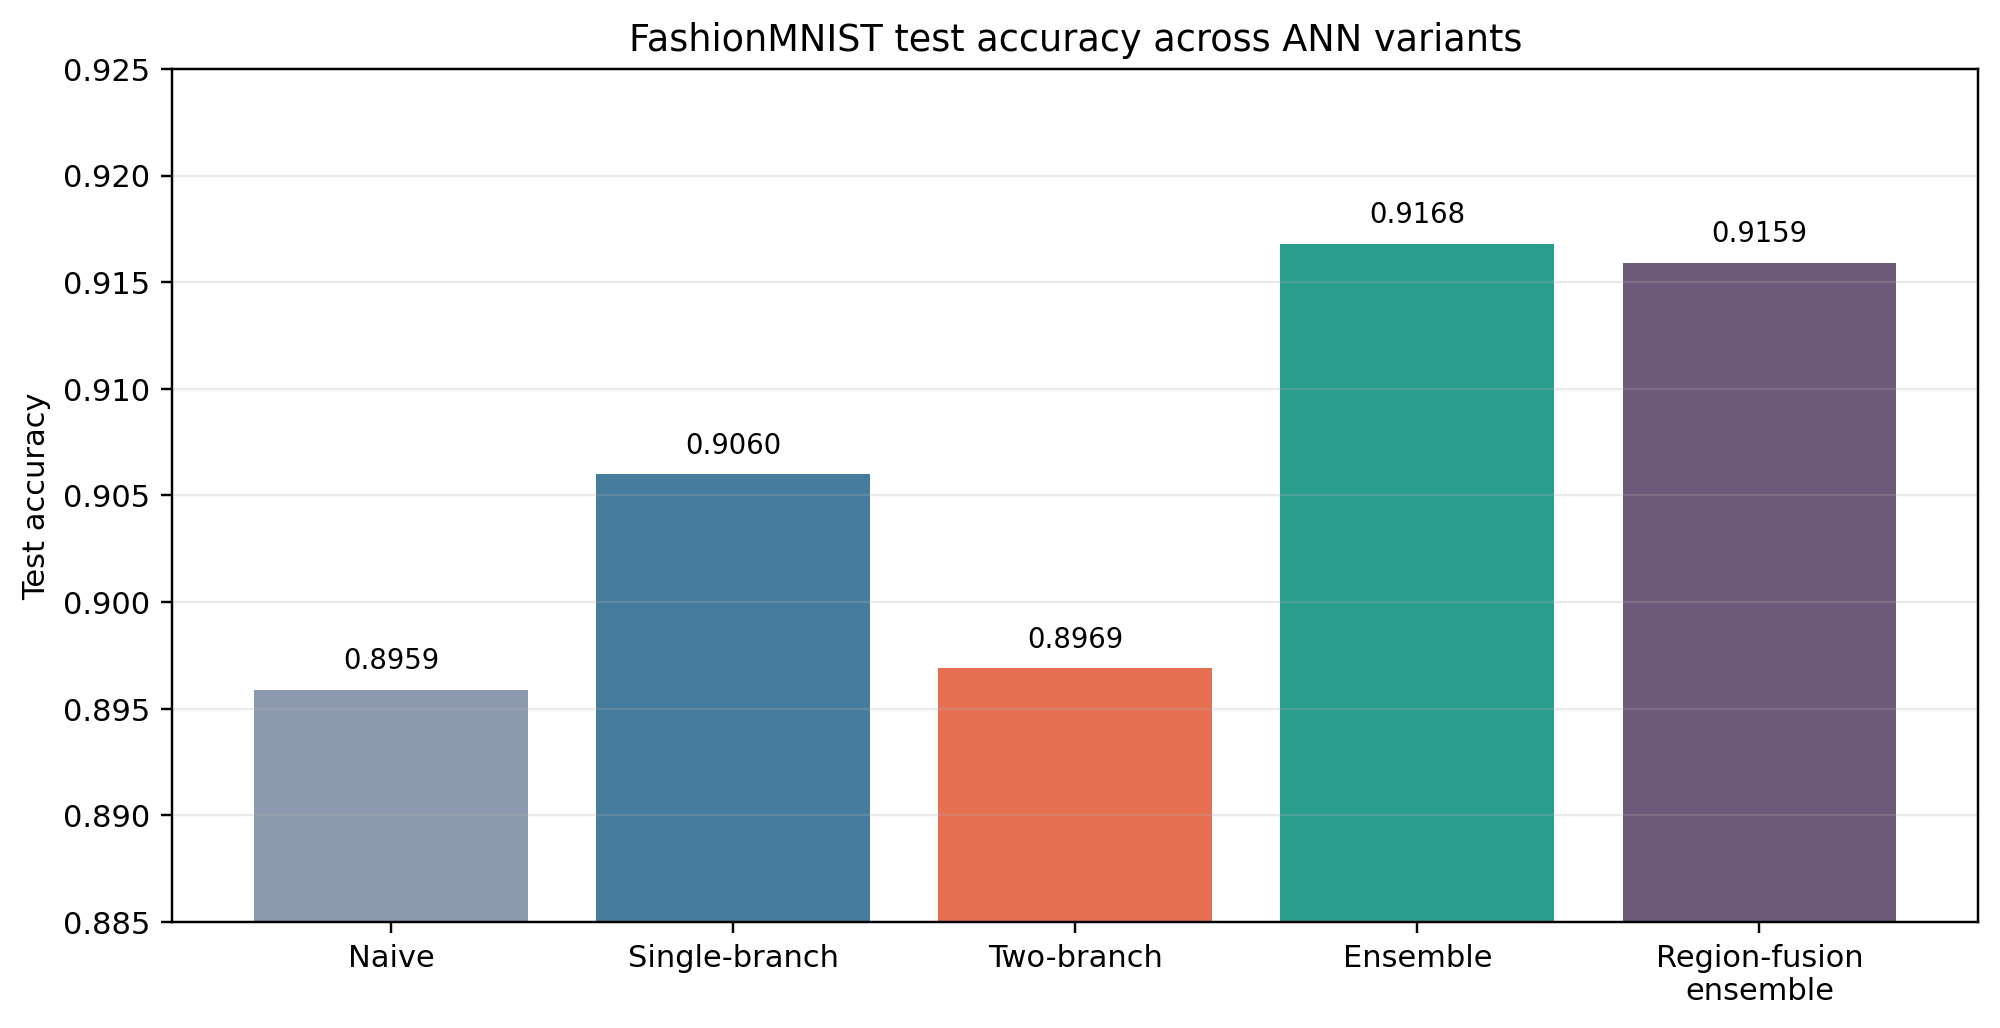
\includegraphics[width=0.95\textwidth]{figures/fashion-mnist-comparison/model_accuracy_comparison.png}
  \caption{So sánh test accuracy giữa các cấu hình ANN trên FashionMNIST.}
  \label{fig:fashion-mnist-model-comparison}
\end{figure}

\begin{figure}[H]
  \centering
  
\includegraphics[width=0.82\textwidth]{figures/fashion-mnist-ensemble/confusion_matrix.png}
  \caption{Confusion matrix của ensemble 3 mô hình single-branch ANN trên FashionMNIST.}
  \label{fig:fashion-mnist-ensemble-confusion}
\end{figure}

\begin{figure}[H]
  \centering
  
\includegraphics[width=0.95\textwidth]{figures/fashion-mnist-ensemble/class_accuracy_bar.png}
  \caption{Accuracy theo từng lớp của ensemble 3 mô hình single-branch ANN trên FashionMNIST.}
  \label{fig:fashion-mnist-ensemble-class-accuracy}
\end{figure}

\begin{table}[H]
\centering
\caption{Các cặp nhầm lẫn lớn nhất của ensemble single-branch ANN trên FashionMNIST}
\label{tab:fashion-mnist-ensemble-top-errors}
\begin{tabular}{l c}
\toprule
Cặp nhầm lẫn & Số mẫu \\
\midrule
T-shirt/top $\rightarrow$ Shirt & 95 \\
Shirt $\rightarrow$ T-shirt/top & 79 \\
Pullover $\rightarrow$ Shirt & 65 \\
Coat $\rightarrow$ Shirt & 63 \\
Shirt $\rightarrow$ Pullover & 59 \\
Shirt $\rightarrow$ Coat & 58 \\
Coat $\rightarrow$ Pullover & 50 \\
Pullover $\rightarrow$ Coat & 44 \\
\bottomrule
\end{tabular}
\end{table}


Ensemble đạt $91.68\%$ test accuracy, cao hơn tất cả các mô hình đơn trước đó. Các cặp nhầm lẫn khó nhất vẫn không biến mất, nhưng số lượng lỗi ở những cặp như \textit{T-shirt/top} $\rightarrow$ \textit{Shirt} hay \textit{Shirt} $\rightarrow$ \textit{T-shirt/top} đều giảm xuống. Điều này cho thấy trên FashionMNIST, vấn đề không phải là một mô hình đơn lẻ không đủ mạnh để học đặc trưng, mà là quyết định cuối còn nhạy với seed và nhiễu của từng lượt huấn luyện; ensemble giúp làm phẳng dao động đó. Nhìn theo benchmark công khai của bộ dữ liệu, đây cũng là hướng cải tiến tự nhiên khi MLP đơn đã chạm trần tương đối rõ~\cite{fashionmnist_repo}.

\subsection{Region-focused feature fusion + ensemble}

Từ kết quả của ensemble single-branch, điểm nghẽn còn lại vẫn tập trung gần như hoàn toàn ở nhóm lớp áo phần thân trên, đặc biệt là \textit{T-shirt/top}, \textit{Shirt}, \textit{Pullover} và \textit{Coat}. Insight rút ra ở đây là HOG toàn ảnh và raw pixel đã mô tả tốt silhouette tổng thể, nhưng chưa nhấn đủ mạnh những khác biệt cục bộ ở cổ áo, vai và độ xòe của tay áo. Vì vậy, biến thể tiếp theo vẫn giữ đúng khung single-branch ensemble để so sánh công bằng, nhưng thay đầu vào bằng bộ đặc trưng giàu thông tin vùng hơn:
\[
2814 = 784 + 1296 + 648 + 16 + 56 + 14,
\]
trong đó $784$ là raw pixel, $1296$ là HOG toàn ảnh, $648$ là HOG của nửa trên ảnh, $16$ là zoning density trên lưới $4 \times 4$, $56$ là row/column projection, và $14$ là upper-width profile. Mục tiêu của thiết kế này là làm cho mô hình nhìn rõ hơn phần thân trên của trang phục, thay vì chỉ dựa vào hình dáng tổng thể của toàn vật thể.

Kiến trúc của mỗi mô hình thành phần vẫn giữ đúng một form MLP đơn để việc so sánh chỉ còn phụ thuộc vào đầu vào:
\[
2814 \rightarrow 1024 \rightarrow 512 \rightarrow 256 \rightarrow 10,
\]
đi kèm BatchNorm, GELU, Dropout$(0.25)$, AdamW, cross-entropy với label smoothing và cosine scheduler. Việc cố ý không đổi phần thân mạng có ý nghĩa rất quan trọng: nếu kết quả thay đổi, có thể quy cải thiện hoặc suy giảm chủ yếu cho bộ đặc trưng vùng thân trên, thay vì do khác biệt về optimizer, regularization hay độ rộng mạng.

\begin{table}[H]
\centering
\caption{So sánh các seed của ensemble region-fusion trên FashionMNIST}
\label{tab:fashion-mnist-region-fusion-seed-comparison}
\begin{tabular}{l c c c}
\toprule
Cấu hình & Final train acc & Test acc & Generalization gap \\
\midrule
Seed 42 & 0.99998 & 0.9064 & 0.0936 \\
Seed 52 & 0.99990 & 0.9109 & 0.0890 \\
Seed 62 & 0.99993 & 0.9102 & 0.0897 \\
Ensemble (3 models) & -- & 0.9159 & -- \\
\bottomrule
\end{tabular}
\end{table}

\begin{table}[H]
\centering
\caption{Kết quả ensemble 3 mô hình ANN với đặc trưng vùng thân trên trên FashionMNIST}
\label{tab:fashion-mnist-region-fusion-results}
\begin{tabular}{l c}
\toprule
Chỉ số & Giá trị \\
\midrule
Test accuracy & 0.9159 \\
Số mô hình trong ensemble & 3 \\
Đầu vào mỗi mô hình & $2814 = 784 + 1296 + 648 + 16 + 56 + 14$ \\
\bottomrule
\end{tabular}
\end{table}


\begin{figure}[H]
  \centering
  
\includegraphics[width=0.82\textwidth]{figures/fashion-mnist-region-fusion/confusion_matrix.png}
  \caption{Confusion matrix của region-focused feature fusion ensemble trên FashionMNIST.}
  \label{fig:fashion-mnist-region-fusion-confusion}
\end{figure}

\begin{figure}[H]
  \centering
  
\includegraphics[width=0.95\textwidth]{figures/fashion-mnist-region-fusion/class_accuracy_bar.png}
  \caption{Accuracy theo từng lớp của region-focused feature fusion ensemble trên FashionMNIST.}
  \label{fig:fashion-mnist-region-fusion-class-accuracy}
\end{figure}

\begin{figure}[H]
  \centering
  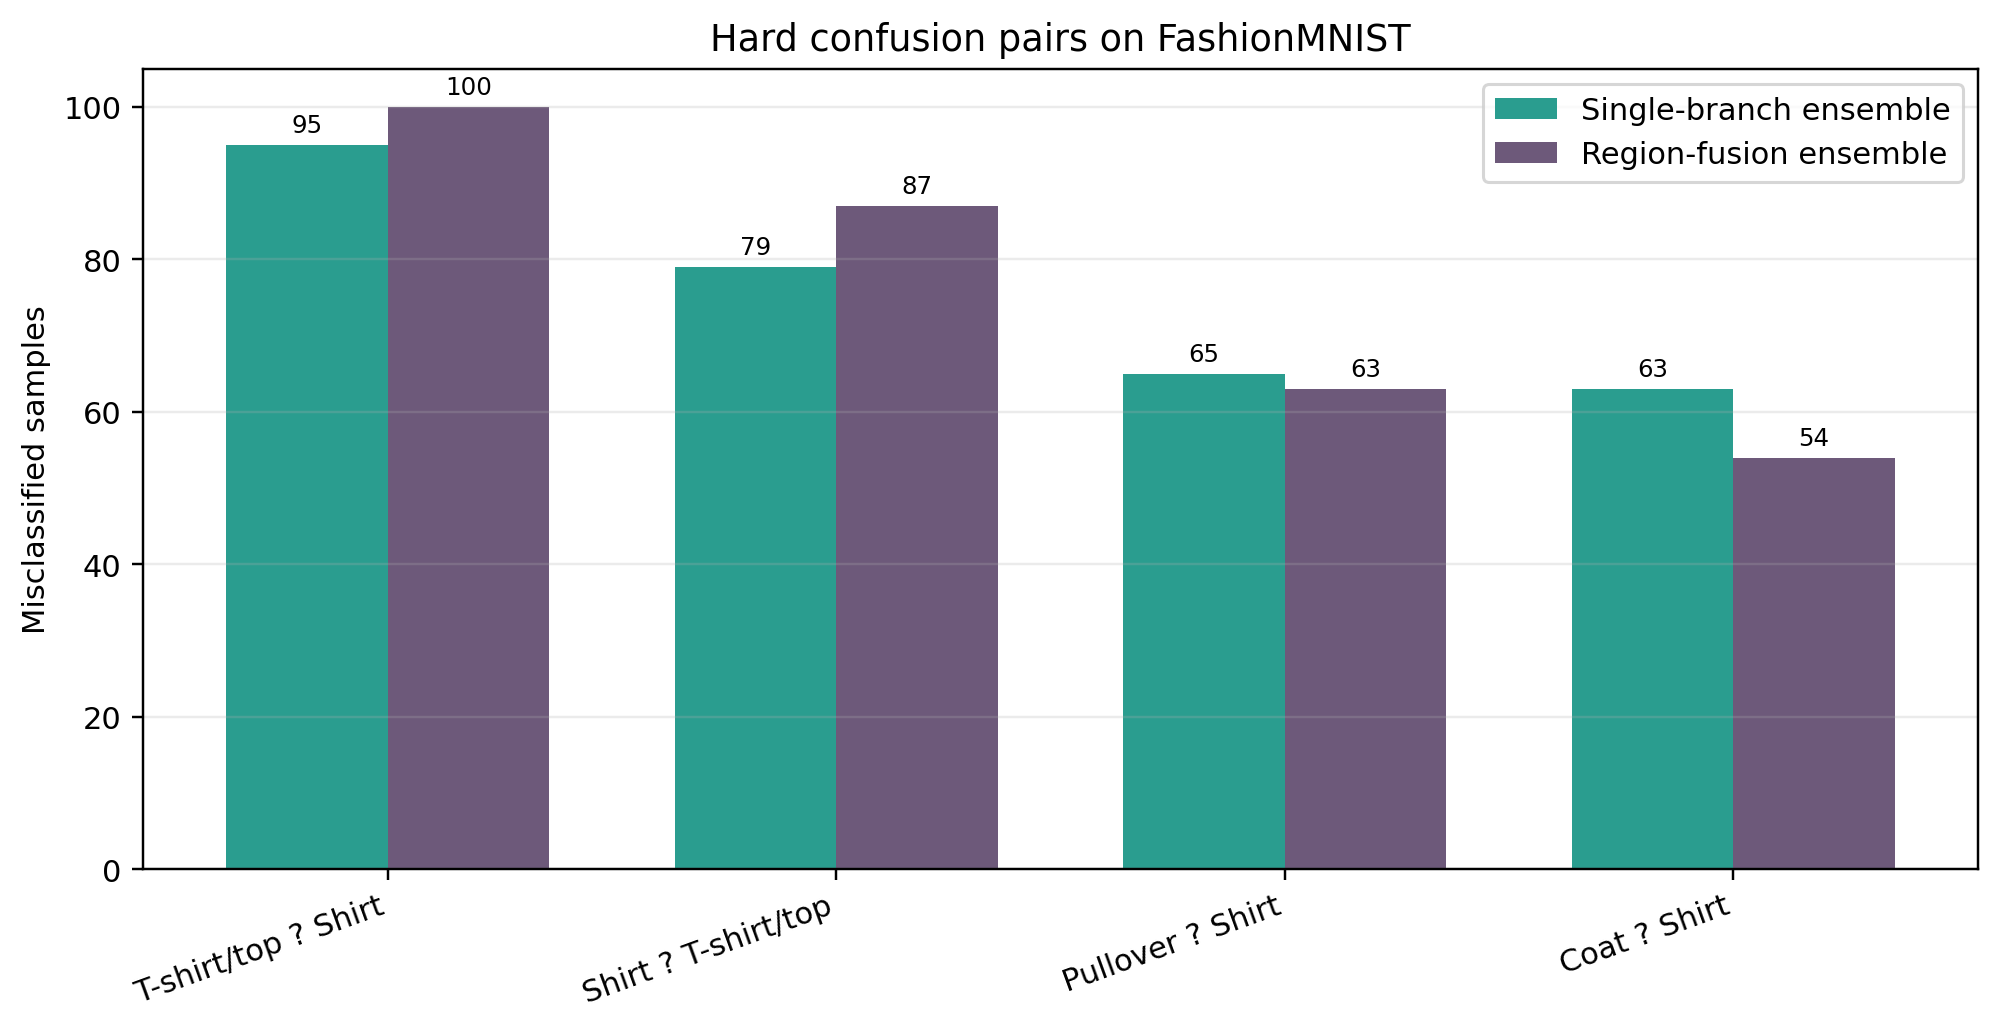
\includegraphics[width=0.92\textwidth]{figures/fashion-mnist-comparison/shirt_confusion_comparison.png}
  \caption{So sánh các cặp nhầm lẫn khó nhất giữa ensemble single-branch và region-focused feature fusion ensemble.}
  \label{fig:fashion-mnist-shirt-confusion-comparison}
\end{figure}

\begin{table}[H]
\centering
\caption{Các cặp nhầm lẫn lớn nhất của region-fusion ensemble trên FashionMNIST}
\label{tab:fashion-mnist-region-fusion-top-errors}
\begin{tabular}{l c}
\toprule
Cặp nhầm lẫn & Số mẫu \\
\midrule
T-shirt/top $\rightarrow$ Shirt & 100 \\
Shirt $\rightarrow$ T-shirt/top & 87 \\
Shirt $\rightarrow$ Coat & 68 \\
Pullover $\rightarrow$ Shirt & 63 \\
Pullover $\rightarrow$ Coat & 54 \\
Coat $\rightarrow$ Shirt & 54 \\
Coat $\rightarrow$ Pullover & 51 \\
Shirt $\rightarrow$ Pullover & 50 \\
\bottomrule
\end{tabular}
\end{table}


Kết quả thu được là $91.59\%$ test accuracy, tức rất sát nhưng vẫn thấp hơn nhẹ so với ensemble single-branch ($91.68\%$). Điều này cho thấy giả thuyết \textit{thêm đặc trưng tập trung vào vùng thân trên sẽ tiếp tục cải thiện kết quả} không được xác nhận trong bộ dữ liệu hiện tại. Thực tế, các cặp nhầm lẫn chính như \textit{T-shirt/top} $\rightarrow$ \textit{Shirt} và \textit{Shirt} $\rightarrow$ \textit{T-shirt/top} không giảm mà còn tăng nhẹ từ $95/79$ lên $100/87$. Nói cách khác, hướng feature engineering này có lý về mặt trực giác, nhưng ở độ phân giải $28 \times 28$ của FashionMNIST, phần thông tin hình học bổ sung ở nửa trên vẫn chưa đủ sạch để vượt qua ensemble single-branch gốc.

\section{Tổng hợp kết quả và nhận xét}

\begin{table}[H]
\centering
\caption{Kiến trúc các biến thể ANN trên FashionMNIST}
\label{tab:fashion-ann-architecture-details}
\small
\begin{tabularx}{\textwidth}{>{\raggedright\arraybackslash}p{3cm} >{\raggedright\arraybackslash}p{3.2cm} >{\raggedright\arraybackslash}X >{\raggedright\arraybackslash}p{3.1cm}}
\toprule
Biến thể & Đầu vào & Kiến trúc & Thành phần chính \\
\midrule
Naive ANN & Raw pixel $784$ & $784 \rightarrow 1024 \rightarrow 512 \rightarrow 256 \rightarrow 10$ & ReLU + fully-connected \\
Single-branch ANN & $2080 = 784 + 1296$ & $2080 \rightarrow 1024 \rightarrow 512 \rightarrow 256 \rightarrow 10$ & BN + GELU + Dropout$(0.25)$ \\
Two-branch ANN & Raw $784$, HOG $1296$ & Raw: $784 \rightarrow 512 \rightarrow 256$; HOG: $1296 \rightarrow 768 \rightarrow 256$; head: $512 \rightarrow 256 \rightarrow 10$ & BN + GELU + Dropout$(0.25)$ \\
Single-branch ensemble & 3 mô hình single-branch độc lập & Trung bình softmax probability của ba seed $42/52/62$ & Ensemble xác suất \\
Region-fusion ensemble & $2814 = 784 + 1296 + 648 + 16 + 56 + 14$ & 3 mô hình $2814 \rightarrow 1024 \rightarrow 512 \rightarrow 256 \rightarrow 10$ & HOG vùng trên + zoning + projection + ensemble \\
\bottomrule
\end{tabularx}
\end{table}

\begin{table}[H]
\centering
\caption{Thông số huấn luyện của các biến thể ANN trên FashionMNIST}
\label{tab:fashion-ann-hyperparameters}
\small
\begin{tabularx}{\textwidth}{>{\raggedright\arraybackslash}p{3cm} >{\raggedright\arraybackslash}p{3.2cm} >{\raggedright\arraybackslash}p{2.2cm} >{\raggedright\arraybackslash}X}
\toprule
Biến thể & Tối ưu hóa & Batch/epoch & Tiền xử lý và augmentation \\
\midrule
Naive ANN & Adam, CE, không scheduler & $256 / 50$ & Chỉ raw pixel, không tiền xử lý bổ sung \\
Single-branch ANN & AdamW, CE+LS, cosine, $wd=10^{-4}$ & $256 / 50$ & Affine; deslant; recenter; HOG \\
Two-branch ANN & AdamW, CE+LS, cosine, $wd=10^{-4}$ & $256 / 50$ & Affine; deslant; recenter; tách raw/HOG \\
Single-branch ensemble & 3 lần chạy single-branch với seed khác nhau & $256 / 50$ mỗi mô hình & Cùng pipeline single-branch; ensemble ở bước test \\
Region-fusion ensemble & 3 lần chạy ANN vùng thân trên với seed khác nhau & $256 / 50$ mỗi mô hình & HOG toàn ảnh + HOG nửa trên + zoning + projection; ensemble ở bước test \\
\bottomrule
\end{tabularx}
\end{table}

\begin{table}[H]
\centering
\caption{Logic chuyển từ một biến thể ANN sang biến thể kế tiếp trên FashionMNIST}
\label{tab:fashion-ann-iteration-logic}
\small
\begin{tabularx}{\textwidth}{>{\raggedright\arraybackslash}p{3.2cm} >{\raggedright\arraybackslash}X >{\raggedright\arraybackslash}X}
\toprule
Biến thể hiện tại & Điểm yếu quan sát được & Ý tưởng cho biến thể kế tiếp \\
\midrule
Naive ANN & Chỉ dựa vào raw pixel nên rất nhạy với silhouette tổng quát và khó tách các lớp áo gần nhau & Thêm deslant, recenter và HOG để bổ sung thông tin hướng nét và hình học \\
Single-branch ANN & Các lớp áo như \textit{Shirt}, \textit{Pullover}, \textit{Coat} vẫn chồng lấn mạnh & Thử tách raw pixel và HOG thành hai nhánh riêng \\
Two-branch ANN & Tách nhánh không cải thiện; test accuracy còn thấp hơn single-branch & Giữ kiến trúc đơn mạnh nhất và giảm phương sai bằng ensemble nhiều seed \\
Single-branch ensemble & Lỗi \textit{Shirt} $\leftrightarrow$ \textit{T-shirt/top}$/$\textit{Pullover}$/$\textit{Coat} vẫn là nút thắt chính & Tăng đặc trưng vùng thân trên để nhấn khác biệt ở cổ áo, vai và tay áo \\
\bottomrule
\end{tabularx}
\end{table}

\begin{table}[H]
\centering
\caption{So sánh các cấu hình ANN trên FashionMNIST}
\label{tab:fashion-mnist-model-comparison}
\begin{tabular}{l c c c}
\toprule
Mô hình & Final train acc & Test acc & Generalization gap \\
\midrule
Naive ANN & 0.9796 & 0.8959 & 0.0837 \\
Single-branch ANN & 0.99997 & 0.9060 & 0.0940 \\
Two-branch ANN & 0.99987 & 0.8969 & 0.1030 \\
Single-branch ensemble & -- & 0.9168 & -- \\
Region-fusion ensemble & -- & 0.9159 & -- \\
\bottomrule
\end{tabular}
\end{table}


Các bảng tổng hợp cho thấy một lộ trình rất rõ. Naive ANN dừng ở mức $89.59\%$, xác nhận rằng raw pixel đơn thuần là chưa đủ cho dữ liệu thời trang. Khi thêm \textit{deslant + recenter + HOG}, single-branch tăng lên $90.60\%$ và trở thành bước cải thiện đầu tiên có ý nghĩa. Two-branch không cải thiện kết quả; ngược lại, nó còn thấp hơn single-branch, nên giả thuyết tách raw pixel và HOG thành hai nhánh riêng không được xác nhận trong bài toán này. Ensemble mới là bước cải tiến thực sự hiệu quả, đưa test accuracy lên $91.68\%$. Biến thể region-focused feature fusion bổ sung thêm thông tin cho phần thân trên của trang phục, nhưng kết quả chỉ đạt $91.59\%$, nên chưa vượt được ensemble single-branch gốc.

Kết luận cho Chương 2 là: với FashionMNIST, thành phần mang lại lợi ích lớn nhất vẫn là giảm phương sai dự đoán bằng ensemble trên biến thể đơn tốt nhất. Những đặc trưng vùng thân trên có hợp lý về mặt trực giác và giúp phân tích lỗi chặt chẽ hơn, nhưng trong giới hạn độ phân giải $28 \times 28$, chúng chưa tạo ra cải thiện thực nghiệm rõ ràng. Vì vậy, cấu hình tốt nhất hiện tại cho FashionMNIST vẫn là ensemble của ba mô hình single-branch ANN, còn region-focused feature fusion nên được xem là một hướng thử nghiệm có cơ sở nhưng chưa đem lại lợi ích đủ thuyết phục để thay thế cấu hình đang dẫn đầu.
